
%% This is a skeleton file demonstrating the use of IEEEtran.cls
%% (requires IEEEtran.cls version 1.7 or later) with an IEEE journal paper.
%%
%% Support sites:
%% http://www.michaelshell.org/tex/ieeetran/
%% http://www.ctan.org/tex-archive/macros/latex/contrib/IEEEtran/
%% and
%% http://www.ieee.org/


\documentclass[conference]{IEEEtran}
\usepackage{blindtext}
\usepackage{graphicx}
\graphicspath{ {images/} }
\usepackage{float}
\usepackage{url}
\usepackage{cite}


\begin{document}
%
% paper title
% can use linebreaks \\ within to get better formatting as desired
\title{Is filecoin a \$257 Million bubble or a pyramid scheme?}
%
%
% author names and IEEE memberships
% note positions of commas and nonbreaking spaces ( ~ ) LaTeX will not break
% a structure at a ~ so this keeps an author's name from being broken across
% two lines.
% use \thanks{} to gain access to the first footnote area
% a separate \thanks must be used for each paragraph as LaTeX2e's \thanks
% was not built to handle multiple paragraphs
%

\author{
\IEEEauthorblockN{Marc Juchli}
\IEEEauthorblockA{Faculty of Electrical Engineering,\\ Mathematics and Computer Science\\
Delft University of Technology\\
m.b.juchli@student.tudelft.nl}
\and
\IEEEauthorblockN{Johan A. Pouwelse}
\IEEEauthorblockA{Parallel and Distributed Systems Group \\ Department of Software and Computer Technology \\
Delft University of Technology\\
j.a.pouwelse@tudelft.nl}
}


% The paper headers
%\markboth{The Culture Clash, September~2016}%
%{}
% The only time the second header will appear is for the odd numbered pages

% make the title area
\maketitle

\begin{abstract}
%\boldmath

...

\end{abstract}

\begin{IEEEkeywords}
filecoin, decentralized storage network, ico, proof-of-spacetime, crypto-currency.
\end{IEEEkeywords}

\IEEEpeerreviewmaketitle

\section{Introduction}

\begin{quote}"A MASSIVE AMOUNT OF STORAGE SITS UNUSED IN DATA CENTERS AND HARD DRIVES AROUND THE WORLD." \cite{filecoin-io}\end{quote}
With this slogan Protocol Labs is about to disrupt the storage market by using \textit{proof-of-spacetime} as their driving source.
The Filecoin project describes a decentralized storage market where anyone, worldwide, is able to participate as a storage provider.
The concept is indeed promising and convinced the investors such that a total of \$257 million had been raised –-- the biggest initial coin offering (ICO) as of today (September 2017).

However, the idea of a decentralized storage market is not a novel concept.
Others\cite{tribler}\cite{mojo-nation} have tried in past too, but yet were not able to scale as much as Filecoin advertises to do, and eventually failed.
More recent projects\cite{storj}\cite{sia} are currently working towards building a similar system with conceptual differences which will be uncovered briefly in this paper.

This paper aims to analyze the ICO launch of Filecoin and reasons about the exceptionally large investment using heavily discussed topics in social media channels.
Further, the feasibility in terms of technical as well as economical design is studied.
We aim to uncover potential weaknesses but also highlight strengths of the proposed white-paper \cite{filecoin}.
The novel \textit{proof-of-spacetime} consensus algorithm is being highlighted and compared with consensus proposals from projects such as StorJ and Sia.
Eventually, the ICO launch is opposed to the \textit{scientific 1975 rule}, a model for pyramid schemes\cite{pyramid-scheme}, and the feasibility is confronted with the \textit{speculative bubble model}\cite{bubble}.

The structure of this paper is as follows: Section \ref{sec:documented-failure} lays out a history of decentralized storage projects with a similar ambition as Filecoin, but that have failed over time. 
Section \ref{sec:recent-competitors} mentions recent competitor projects that make use of a blockchain.
The following Section \ref{sec:ico-analysis} is an introduction to the Filecoin project by analyzing the ICO including the reasoning about the token sale and allocation thereof.
Section \ref{sec:tech-feasibility} reasons whether the promises of the Filecoin project are technically feasible, whereas Section \ref{sec:eco-feasibility} questions its economical feasibility.


\section{15 years of documented failure}
\label{sec:documented-failure}

In July 2000, long before the blockchain era, the Mojo Nation software \cite{mojo-nation} was released, aiming to serve an "emergent file store" to its users.
The project successfully deployed a decentralized storage network in an environment consisting of unmanaged nodes.
It used consistent hashing \cite{consistent-hashing} to locate nodes and data blocks.
However, the project was shut down in February 2002 due to a number of problems:
\begin{itemize}
\item Data Availability: the main issue was the inconsistency of data available to its users as it depended upon which server nodes were connected at the given time.
According to Maymounkov et al.\cite{peer-to-peer-xor} this could have been avoided by heuristically favoring long-lived nodes and by discriminating newly joined nodes which show a frequent join- and leave behaviour.
\item Firewalls and NAT: networking hurdles such as firewalls and network address translation (NAT) prevented a substantial amount of nodes to act as servers.
\item Mutual distrust: in order to have a network of nodes to behave as designed a \textit{motivation to cooperate} needs to be established within the network, combined with sophisticated \textit{attack resistance} mechanism which prevents nodes from using resources of other nodes without offering equal amounts of services in return.
\end{itemize}
\hfill
\\
Also academia has been struggling to succeed in building self-organizing systems.
Tribler\cite{tribler} is based on robust reputation and craft collaboration, an environment where one could think of a decentralized marketplace which can handle storage as an asset.
The 12 years of development has been a history affected by many hurdles.
Security issues such as collusion attacks\cite{tribler-hurdles} have slowed down the development progress enormously, preventing the project to scale.

\section{Recent Competitors}
\label{sec:recent-competitors}
At the time of writing this paper, an invasion of ICOs has arisen, among some of which are projects that tend to go into a similar direction as Filecoin does.
Figure \ref{fig:ico-vs-venture} shows that the funds invested in ICOs has overcome the investments made in the venture capital sector.
\begin{figure}[h]
\centering
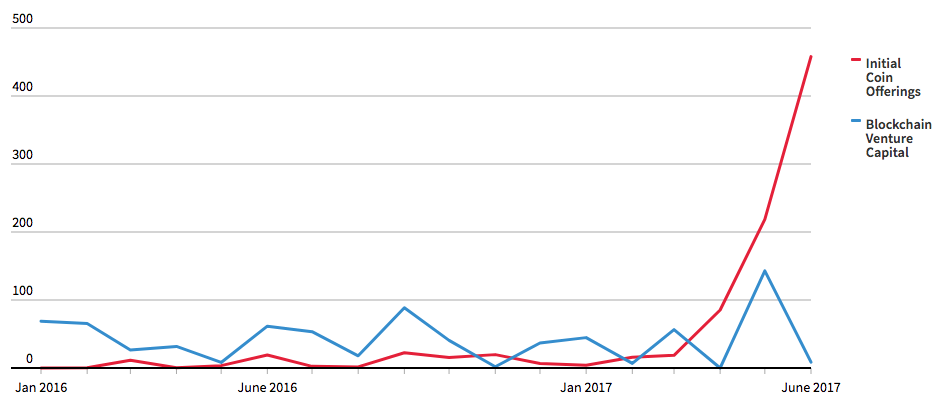
\includegraphics[width=0.45\textwidth]{ico-vs-venture}
\caption{ICOs vs Venture Capital \cite{ico-vs-venture}}
\label{fig:ico-vs-venture}
\end{figure}
Primary examples of decentralized, incentivized, byzantine fault-tolerant storage networks which shall be competitive with centralized alternatives such as Amazon S3\cite{amazon-s3} are: StorJ\cite{storj}, Sia\cite{sia} and MaidSafe\cite{maidsafe}.
\begin{itemize}
\item \textbf{Sia}: supports on-blockchain smart contracts which define payments for hosts while providing storage. 
Payment is guaranteed once the contract has been created and ensures that the host is being paid in case the the uploader never accesses the file. 
Additionally, the contract enforces penalties for hosts which go offline or lose data.
\item \textbf{Storj}: is similar to Sia but does not feature on-blockchain storage contracts but instead offers a pay-as-you-go model for nodes who provide storage. 
Once the host disappears or goes offline, payments are halted.
\item \textbf{MaidSAFE} goes beyond decentralized storage with a less sophisticated focus on efficiency.
MaidSAFE uses a novel scheme for achieving consensus by not relying on a blockchain but instead on close group consensus and hence is not proof-of-work related.

\end{itemize}

\section{ICO analysis}
\label{sec:ico-analysis}

The Filecoin ICO started on August 10, 2017 and closed the offering on September 7th.
It was the first ICO ever which complied with SEC securities regulations and hence only accredited investors were allowed to contribute (Reg. D, 506(c), see \cite{regulation-506}).
Further was the ICO conducted using CoinList\cite{coinlist}, a platform for token sales, built by Protocol Labs too.
CoinList partners with AngelList\cite{angellist} whose responsibility is on the compliance side regarding the law.
In total, approximately \$257'000'000 was raised, formed of \$52'000'000 from presale and \$205'800'000 Reg D investments.
For the latter category, \$135 million was raised within the first hour.

\subsection{Simple Agreement for Future Tokens}
The tokens distributed during the ICO were so called Simple Agreement for Future Tokens (SAFT). 
This instrument allows Coinlist to distribute investors the \textit{right} to receive units of the actual Filecoin tokens (FIL) in the future.
The definiton of SAFT, however, is also equipped with the following statement:
\begin{quotation}
"...a significant portion of the amount raised under the SAFTs will be used to fund the Company’s development of a decentralized storage network that enables entities to earn Filecoin (the “Filecoin Network”)".\cite{saft-agreement}
\end{quotation}
Therefore, it is not explicitly mentioned to what extent the development process is being funded, and thus it is left to be decided by Protocol Labs Inc., solely.
Additionally, SAFT introduces great flexibility to the token intermediary, CoinList, as the agreement not only allows to verify accredited investors but also to specify \textit{events} transparently.
Transparency is certainly appreciated when funds are being transferred, but it is needless to say that the terms have to be fully understood by both parties.
One such event, which might be underestimated by the investor, is the \textit{Dissolution Event} and is defined as follows:
\begin{quotation}
"Dissolution Event means (i) a voluntary termination of operations of the Company, (ii)
a general assignment for the benefit of the Company’s creditors or (iii) any other liquidation,
dissolution or winding up of the Company, whether voluntary or involuntary."\cite{saft-agreement}
\end{quotation}
Knowing that it is at any given time possible for Protocal Labs to terminate their business, the entire setup of the ICO becomes fragile when reading the \textit{execution plan}:
\begin{quotation}
"If immediately prior to the consummation of the Dissolution Event, the assets of the Company that remain legally available for distribution to the Purchaser and all holders of all other SAFTs (the “Dissolving Purchasers”), as determined in good faith by the Company’s board of directors, are insufficient to permit the payment to the Dissolving Purchasers of their respective Returned Purchase Amounts, then the remaining assets of the Company legally available for distribution will be distributed with equal priority and pro rata among the Dissolving Purchasers..."\cite{saft-agreement}\end{quotation}
After all, only the \textit{remaining} assets which are legally available will be distributed in the case of a \textit{Dissolution Event}; including definition (i), the voluntary termination.
Unfortunately, if one considers the worst case scenario in which Protocol Labs decides to terminate the operation, while having spent all the funds available, the investors would likely be excluded from the distribution of any reward.
Similarly, if the project does not announce a \textit{Network Launch}\cite{saft-agreement} event by July 18, 2022 (including a 60-days extension), then, by definition (i) or (iii), investors would have to expect a \textit{Dissolution Event} to be announced as a subsequent step.

\subsection{Token allocation}
As presented in \cite{token-sale}, the allocation of the Filecoin token is distributed to 4 groups of participants:
\begin{itemize}
\item 70\% to Filecoin Miners as mining block rewards once \textit{Network Launch} is past
\item 15\% to Protocol labs as genesis allocation with 6-year linear vesting
\item 10\% to Investors as genesis allocation with 6 months to 3 year linear vesting
\item 5\% to the Filecoin Foundation as genesis allocation with 6-year linear vesting
\end{itemize}
The total of \$257 million US-dollar raised during the advisor pre-sale and investor sale (see \ref{subsec:token-sale}) therefore only accounts up to 10\% of the total coins expecting to be circulating after several years past \textit{Network Launch}.
Since the half-life time of Filecoin block rewards is set to 6 years, this will likely not change significantly for several years, considering that the \textit{Network Launch} requires a solid implementation of the Filcoin ecosystem.

\subsection{Token sale}
\label{subsec:token-sale}
The offering of SAFTs was established in a two-phase process: the first phase allowed Protocol Labs as well as Filecoin advisors to purchase SAFTs prior the broader group of investors. 
The latter were able to proceed purchases in a second phase.
In the first phase, the price was fixed at 0.75 USD/FIL.
For the second phase, a pricing function was introduced:
\[ price = max(\$1, \frac{amountRaised}{\$40'000'000}) \]
The pricing function increases linearly with the amount being raised, as indictated in Figure \ref{fig:sale-price}.
\begin{figure}[h]
\centering
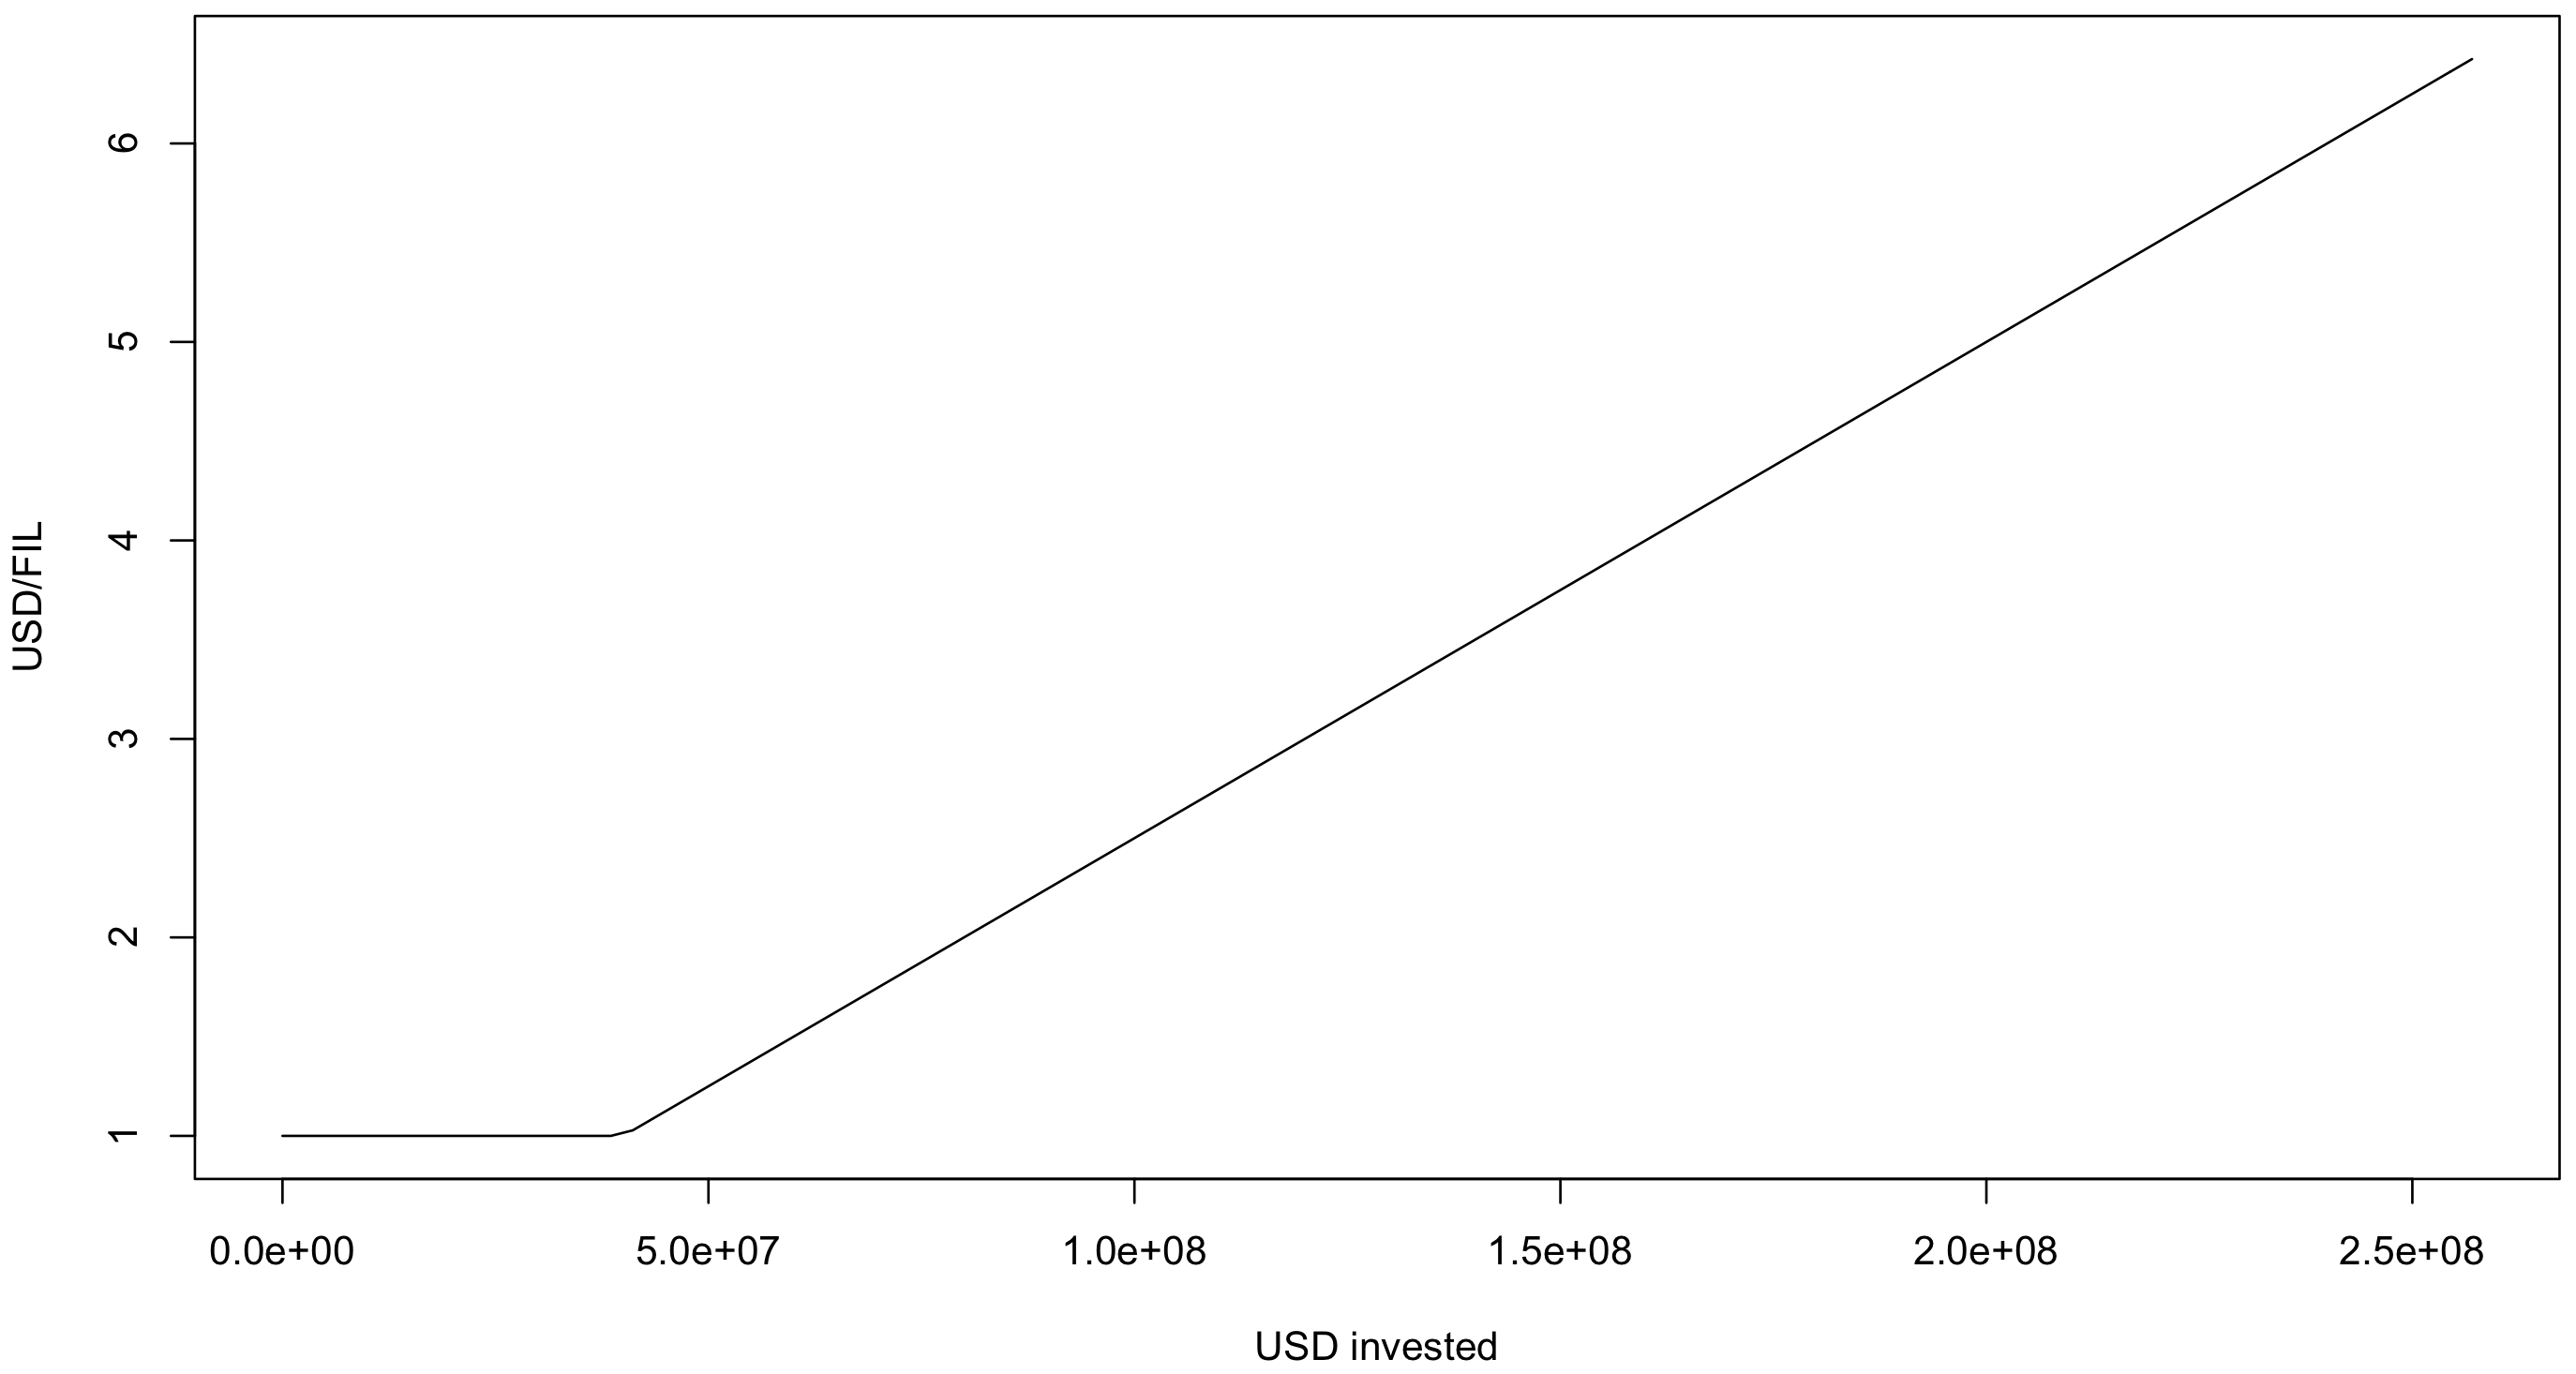
\includegraphics[width=0.45\textwidth]{filecoin-tokensale.png}
\caption{Filecoin sale price function}
\label{fig:sale-price}
\end{figure}
As a result, the closing price, past \$257'000'000 investments, can be estimated to be approximately \$6.425.
Hence, advisors and Protocol Labs Inc. itself were able to purchase for a price which is a factor of 8.57 lower than the late investor.

\subsection{Questioning investors exclusion}


\section{Is the design technically feasible?}
\label{sec:tech-feasibility}
In this section, technical details will be highlighted with reasoning whether the decisions stated in the Whitepaper\cite{filecoin} are chosen appropriately or arise potential weaknesses.
We further aim to make comparisons to more recent decentralized storage projects involving a blockchain, such as StorJ \cite{storj} and Sia \cite{sia}.

\subsection{Decentralized Storage Network}
\label{subsec:dsn}
The notion \textit{Decentralized Storage Network} (DSN) is a scheme with associated protocols that enables to aggregate and provide data in decentralized coordination manners.
The protocols verify that involved parties execute their operations securely and therefore allows coordination without a trusted party.
The Filecoin DSN introduces three types of participants: (1) \textit{Clients} who pay FIL tokens to store and retrieve data, (2) \textit{Storage Miners} who pledge FIL tokens as a collateral while providing storage which is worth equal amounts of FIL and are eligible to mine new tokens by doing so, and (3) \textit{Retrieval Miners} who serve data upon client requests, and oftentimes act as Storage Miners too.
Further does Filecoin personify all the participating parties which run a \textit{full nodes} as \textit{The Network ($N$)}.
Hence, the protocol scheme is being castellated as a tuple in a very suitable and abstract definition: \texttt{(Put, Get, Manage)}.
Storing and retrieving data is done by Clients using the Put, or respectively Get, Protocol.
The Network is being coordinated using the Manage protocol, which serves to control the available storage, audit offered services by Storage Providers and repair possible faults.
Little is known about the details of \texttt{Manage.AssignOrders} and \texttt{Manage.RepairOrders}, such as, whether the manage protocol follows incentive and rewards nodes for actively maintaining the network.
However, from what is known, the Filecoin DSN, compared to the competitors described in Section \ref{sec:recent-competitors}, is indeed conceptually splendid.
The simplicity of \texttt{(Put, Get, Manage)} implicitly covers additional client operations operations such as \texttt{PING} and \texttt{FIND\_NODE}, as defined in StorJ \cite{storj}.

The flow of storing data, initiated by a client, involves the data to be split into \texttt{pieces} in order to be stored within \texttt{sectors} as part of the disk space provided by storage miners.
Conceptually, the data handling is very similar to StorJ\cite{storj} where data, after it underwent AES256-CTR encryption executed by the client, is split into \textit{shards}.
While StorJ dynamically adjusts the size of the shards depending on the file to be stored, it is yet not known how Filecoin will approach the splitting into pieces.
Filecoin, like StorJ, delegates the encryption task to the client.
However, whereas StorJ enforces encryption in its reference client implementation, Filecoin currently has no plan for offering built-in encryption and leaves this responsibility solely to the client before approaching the Filecoin network.
In order to introduce redundancy for the to be stored data, Filecoin neatly introduces a \textit{replication factor} to be choosen during the \texttt{Put} protocol which allows to increase the tolerance of storage faults.
In contrast, StorJ herefore uses a distinctive \textit{mirror} method.

The guarantees and requirements laid out by the Filecoin DSN can be summarized as follows:
\begin{itemize}
\item \textit{Integrity:} In order to ensure that clients do not accept altered or falsified data, cryptographic hashes are used as a naming convention and serve as identifier for data retrieval (\texttt{Get} protocol) and verification of its content.
Filecoin does not rely on any meta data, such as its competitor StorJ\cite{storj}, but relies on the hash only.
\item \textit{Retrievability:} after the data is successfully stored, clients are ensured that the very same data can eventually be retrieved.
The $(f, m)-tolerant$ system specifies that given $m$ storage miners, a maximum of $f$ faults are tolerated.
Increasing the replication factor hence implicitly increases the chances of recovery.
\item \textit{Public Verifiability and Auditability:} as storage miners are obligated to submit proofs of storage (see \ref{subsec:pos} to the blockchain, any user can verify their validity without having access to the data.
Since \textit{proof-of-spacetime:} implicitly guarantees the continuous existence of the data on the storage miner side, no challenge-response communication is required.
Compared to StorJ\cite{storj}, the communication overhead is therefore reduced while providing the same guarantees.
\item \textit{Incentive compatibility:} like any of the projects mentioned in \ref{sec:recent-competitors}, Filecoin enforces incentive by rewarding parties which store data and punishing those who loose data.
\item \textit{Confidentiality:} as mentioned earlier in this Section, Filecoin is weaker in terms of confidentiality as it fully delegates the encryption task to the client.
\end{itemize}

% Partitioning vs erasure codes \cite{sia}

\subsection{Ledger}
\label{subsec:ledger}
The \texttt{Ledger $L$} being used in Filecoin will be represented by a native blockchain, as announced in \cite{filecoin-investor-faq}, and supports various types of data structures.
The state of the DSN is stored within an \texttt{AllocTable}, which keeps track of \texttt{pieces} and their assigned \texttt{sectors}.
The \texttt{Orderbook} is responsible for storing \texttt{Orders} which either state a request to store data (\texttt{Bid order}), offer a service (\texttt{Ask order}) or confirm a match of bid- and ask orders in form of a \texttt{Deal order}.
Lastly, a \texttt{Pledge} engraved in the ledger represents the collateral of the storage miner in order to accept orders from the clients, as described in \ref{subsec:dsn}.
In contrast, Sia only stores storage contracts which define the terms of the formed agreement between parties and therefore relies on a variant of the Bitcoin protocol\cite{bitcoin}.
As Filecoin is clearly more diverse in terms of data structures additional complexity in the clients is to be expected.
From another perspective, this decision might allow to extend the protocol more easily as the ledger is already lied out to handle various types of data structures.
Having a native blockchain further was a necessary decision in order to employ Proof-of-Spacetime, see \ref{subsec:pos}.
However, by not relying on the Ethereum Network \cite{ethereum} as previously planned and announced at DEVCON2 \cite{devcon2}, and its absence of an ERC20 token \cite{erc20} hence prevents direct compatibility to Ethereum and therefore requires a bridge of some sort.

%\subsection{Fault tolerance}

\subsection{Proof-of-Spacetime}
\label{subsec:pos}
The white-paper\cite{filecoin} describes a novel consensus protocol: \textit{Proof-of-Spacetime} (PoSt).
With Proof-of-Spacetime it becomes possible to check if a prover is storing data for a range of time, or formally:
\begin{quotation}
"A \texttt{PoSt} scheme enables an efficient prover \texttt{P} to convince a verifier \texttt{V} that \texttt{P} is storing data \texttt{D} for some time \texttt{t}."\cite{filecoin}
\end{quotation}
It takes advantage of the capabilities of \textit{Proof-of-Storage}\cite{proof-storage}, which can confirm if a storage provider is storing data at the time of the challenge, by sequentially generating such proofs and recursively compose the executions thereof.
The concrete implementation of Proof-of-Storage is described as \textit{Proof-of-Replication} (PoRep), a novel concept that lets a storage miner to convince a client that its data has been replicated to a uniquely dedicated physical storage.
Other Proof-of-Storage schemes such as Provable Data Possession (PDP)\cite{proof-possession} and Proof-of-Retrievability (PoR)\cite{proof-retrievability} essentially guarantee possession of some data at the time of the challenge/response.
Proof-of-Replication, however, improves those schemes by preventing \textit{Sybil Attacks, Outsourcing Attacks}, and \textit{Generation Attacks}.
As Proof-of-Spacetime is based on Proof-of-Replication, these properties are inherited.
Thus, PoSt prevents pretentious copies which are not physically stored (\textit{Sybil Attack}).
It further denies storage miners to offer more storage than physically available (\textit{Outsourcing Attack}) and also protects from on-demand data generation while this should effectively be stored on a physical disk (\textit{Generation Attack}).
The cryptographic building blocks of PoRep and PoSt rely on zero-knowledge Succinct Non-interactive Arguments of Knowledge (zk-SNARKs).
Zero knowledge proof, including zk-SNARKs have shown to have great potential allowed to build large scale projects such as ZeroCash\cite{zcash}. 
\\
\\
Apart from the extensive capabilities in terms of storing data, Proof-of-Spacetime attempts to reduce resource waste, by considering that storing users data is a form of work.
It is therefore a consensus protocol based on \textit{useful work}.
The usefulness implies that computational power is not wasted--- as this is the case for \textit{Proof-of-Work}\cite{bitcoin} and other consensus algorithms.
In Filecoin, the voting power (the probability of a miner being elected to create a new block) increases proportionally with the storage offered to the network in relation to the storage resources of the entire network.
Due to the fact that Proof-of-Spacetime composes  Proof-of-Replication executions sequentially, it is further considered as non-parallelizable and thus greater computational resources will not have any noticeable effect. \cite{filecoin}

However, given that storage miners may offer varying amounts of storage results, their influence on the network is being distributed continuously and unequally.
Hence, a naive Byzantine Fault Tolerance approach that uses the number of faulty nodes is in the case of Filecoin not a sufficient measure for determining the outcome of a protocol.
Instead, Filecoin proposes \textit{Power Fault Tolerance} (PFT)\cite{filecoin-pft}, an abstraction that defines byzantine faults in terms of the \textit{influence} of a participant.


\subsection{Decentralized Markets}
\label{subsec:markets}
Filecoin introduces two types of markets, \textit{Storage Market} and \textit{Retrieval Market}, represented by two independent, decentralized exchanges.
The notion \textit{Verifiable Markets} is presented and describes a market where participants are able to verify the exchange between buyers and sellers.
Specifically, the protocol describes a two-phase process: \textit{Order matching} allows participants to add buy and sell orders to the orderbook and eventually allows to create deal orders once the two opposite (buy and sell) orders have matched.
The second phase, described as \textit{Settlement}, involves the network to ensure the correct execution of the transfer of goods (data) and eventually initializes a payment.
The \textit{Verifiable Market Protocol} applies to both of the aforementioned markets.\cite{filecoin}
\\
\\
The main purpose of the Storage Market is for clients to request storage and for storage miners to offer their resources. 
Bid- and ask orders from those parties will be placed into an orderbook and are therefore publicly available to any participant of the network.
Filecoin states that "every honest user has the same view of the orderbook".
That is, the orderbook is a data-structure incorporated in the blockchain.
Hence, orders are added to the blockchain if they are valid.
As the Storage Market is a \textit{verifiable market}, orders of type \textit{bid, ask} and \textit{deal} can be validated by every participant.
\\
\indent
The only security related parameter required in the order matching phase is a field (\texttt{ts}) which describes the duration of how long a \textit{deal order} is valid.
This prevents a client from holding back data once the storage miner has committed its resources.
The settlement phase further involves the storage miner to seal their sectors and submit the generated proofs of storage to the blockchain.\cite{filecoin}
\\
\\
The retrieval markets sole purpose is for retrieval miners to provide data to the clients upon their requests.
One very challenging requirement for this market is the \textit{fast} retrieval of data.
Therefore, and unlike the storage market, the retrieval market maintains an off-chain orderbook that allows clients and retrieval miners to find each other.
The absence of a blockchain acting as a trusted party introduces the need for other ways of forming trust between client and retrieval miners.
Filecoin essentially relies on token exchange as trust instrument.
The to be delivered data is being split in multiple pieces and for every successful exchange of a piece the client pays the miner.
If one of the involved parties does not come after its duties, the other party is free to stop.
\\
\indent In order to process payments in the first place a network of payment channels is required.
Filecoin has not stated more detailed plans of how to integrate payment channels into the retrieval market. 
Although this being a risk, much research has been done and promising projects have evolved \cite{lightning}.
\\
\indent The order matching phase of the verifiable market protocol differs much, compared to the storage market.
Since the orderbook cannot be recorded in a blockchain, clients and retrieval miners have to \textit{gossip} their orders.
Filecoin assumes that this point that there is always at least one honest retrieval miner.
\cite{filecoin}

\section{IPFS}
As described in \cite{filecoin}, Filecoin serves as an incentivized seeding layer on top of the InterPlanetary File System (IPFS)\cite{ipfs-whitepaper}.
The Filecoin project is therefore beneficial to IPFS as it intends to add more storage to the network. At the same time, is strongly depending on the technical capabilities and robustness of IPFS.
This sections aims to highlight the capabilities of IPFS and explains the conceptual decisions made while building a peer-to-peer hypermedia protocol.
The latter involves a brief overview of the libp2p project\cite{libp2p}, a modular peer-to-peer networking stack.
Lastly, we reason about possible approaches on how to integrate IFPS in Filecoin.

\subsection{The flaws of HTTP}
The Hypertext Transfer Protocol (HTTP) can be seen the global information protocol that standardized how people distribute and present information among each other.
Publishing content with HTTP is nowadays almost free and led to great birth of innovation and has been driven innovation, economics and culture ever since.
However, the way this valuable content is being distributed a significant flaw: HTTP allows content to \textit{erode} \cite{http-obsolete}.
Covered by \textit{error code 404}\cite{http-rfc}, HTTP fails to maintain links between websites and allows valuable content to vanish completely.
The main reason for this problem to occur are centrally managed servers, free to shut down at any given time.
While short-term availability of content tends to be sufficient, the ongoing erosion of data lacks to maintain long-term availability and results in a vast amount of broken links\cite{broken-links}.
HTTP naturally empathized large organizations to centralize their services which constitutes in an ever increasing potential loss of data.
As a result, what used to be a decentralized web is now moving towards a more and more centralized web structure.
%TODO: figure centralized vs decentralized vs distributed

\subsection{Distributed file system}
\label{subsec:ipfs-dfs}
According to the readme\cite{ipfs-github}: "IPFS is a distributed file system that seeks to connect all computing devices with the same system of files."
In practice, IPFS is a peer-to-peer distributed system that connects all networks using the same system of files. 
The files are version controlled and represented with their hash and as opposed to HTTP, where content is being searched by location, IPFS searches by content.
Hence, IPFS is a content-addressable peer-to-peer hypermedia distribution protocol.

\textit{Nodes}, which are incentiviszed to remain the same and loose network benefits otherwise, are identified by a cryptographic hash of a public-key.
IPFS does not rely on a particular hash function format but instead uses the multihash\cite{multihash} format such that any well-established cryptographic hash function can be used in order to create a node.

The \textit{Network} then allows nodes to communicate while providing a framework which ensures any client, no matter what network stack looks like, can participate.
That is, the client can use any transport protocol and IPFS provides reliability functions if the underlying network does not provide so. 
Connectivity is enhanced using ICE NAT traversal techniques \cite{ice-nat} which for example also includes relaying such that nodes can find nother nodes on their behalf to provide demanded content.
Further more, IPFS does not rely on IP only but instead uses the multiaddr\cite{multiaddr} format to express addresses and their protocols.

\textit{Routing} is required for nodes to find other peers which can serve objects.
A \textit{distributed sloppy hash table (DSHT)}\cite{dsht} serves those purposes and is based on S/Kademlia\cite{kademlia} and Coral\cite{coral}. 
Again, IPFS remains true to its flexible and modular structure and thus allows to change the implementation of \texttt{IPFSRouting} interface, allowing, for example, in a local environment to use a regular hash table. \cite{ipfs-whitepaper}

Proceeding a \textit{block exchange} for distributing data in IPFS is implemented with BitSwap\cite{bitswap}, a protocol inspired by BitTorrent\cite{bittorrent}.
BitSwap is incentivized as it uses a credit system where peers track their balance with other nodes and sending blocks to debtor peers is implemented with probabilistic approach.
Hereby, an additional timeout is being applied in case a sender does not come after its duties, which prevents gaming the probabilities.
Whereas BitTorrent uses tit-for-tat strategy, BitSwamp relies on a debt ratio factor: \[r=\frac{bytes\_sent}{bytes\_received+1}\]
A probabilistic function further describes the likelihood of a peer sending data as follows:
\[P(send|r)= 1-\frac{1}{1 + exp(6-3r)}\]
The function implies that once the debt ratio of a peer surpasses twice the amount of its credit, the likelihood of sending and hence its trustworthiness drops radically.
As a result, this BitSwamp implements a measure of trust using the debt ratio factor and therefore provides resistance against Sybil attacks and values successful relationships among peers yet with the tolerance of temporary unavailability. \cite{ipfs-whitepaper}

In order to effectivly store and distribute blocks in quick and robust manners, IPFS introduces the \textit{Merkle DAG}.
The directed acyclic graph is built-up with cryptographic \texttt{links} of the underlying objects.
The \texttt{object} is a data structure consisting of a \texttt{name}, \texttt{multihash} and \texttt{size}, allowing any type of data to be represented with.
The Merkle DAG, described as "a generalization of the Git data structure"\cite{ipfs-whitepaper}, hence provides properties including: Content Addressing (content is uniquely identified by its multihash checksum), Tamper resistance (content is verified with its checksum) and Deduplication (objects with exact same content are equal and are stored only once). \cite{ipfs-whitepaper}
Allowing to traverse the Merkle DAG is being enabled with UNIX-like paths describing the multi-hashes of the object:\\
\texttt{/ipfs/<hash-of-object>/<name-path-to-object>}
That is, IPFS makes an attempt to reuse long established file system properties while handling data with a fundamentally different concept than what was known so far.

At last and in order to make IPFS a fully useful file system, IPFS introduces IPNS\cite{ipns}, the InterPlanetary Naming System.
The goal is to maintain the Merkle DAG containing immutable content-addressed objects, and apply \textit{Naming} by using mutable pointers to the Merkle DAG.
Thus, enabling user friendly naming. \cite{ipfs-whitepaper}

\subsection{Libp2p}
The development of IPFS has been a demanding challenge in understanding the internet network stack. \cite{libp2p-github}
As a result, the \texttt{libp2p} library was created in order to bundle protocols used for building large scale peer-to-peer applications.
Thus, libp2p can be regarded as an entire network stack, represented by a protocol suite.
Conceptually, libp2p is structured according to Figure \ref{fig:libp2p-stack}.
\ref{fig:sale-price}.
\begin{figure}[h]
\centering
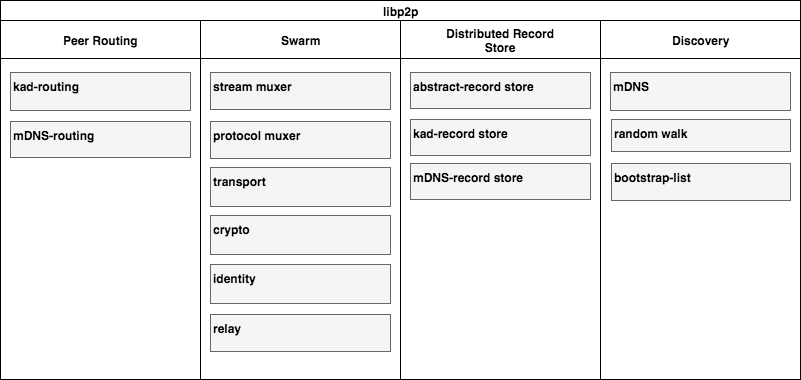
\includegraphics[width=0.45\textwidth]{libp2p-short.png}
\caption{Libp2p network stack}
\label{fig:libp2p-stack}
\end{figure}

The interfaces can be described as follows:
\begin{itemize}
\item \textbf{Peer Routing:} Identifies the peers to which a message should be routed to.
The implementations include \textit{kad-routing}, a kademlia routing table where each peer holds a set of k-buckets; and mDNS-routing which identifies local area network peers.
\item \textbf{Swarm:} handles everything related to the opening of a stream.
A \textit{stream muxer} multiplexes connections per peer and streams per connection.
The \textit{protocol muxer} enables multiplexing of transport protocols on applications level.
This allows several protocols to be muxed in the same socket and therefore only one NAT traversal would be required, if any.
Further more, \textit{Relay} provides an end-to-end encrypted connection where a node asks another node to connect on its behalf and thus can overcome NAT traversal.
\item \textbf{Distributed Record Store:} The aim is to store and distribute records, that is, similar to DNS as it is used for signaling links, announcing peers and content.
The record store was further modularized under the name: IPRS, InterPlanetary Record Store \cite{iprs}.
The interface provides record stores for abstract records, kademila routing records as well as mDNS routing records. 
Having such a record keeping system allows content to be verified by any user of the record store.
\item \textbf{Discovery:} in order for peers to find and identify each other in the network, libp2p provides several ways to do so.
LAN discovery is being implemented with \textit{mDNS}, \textit{Random Walk} using a DHT (distributed hash table) discovery by proceeding random queries enables discovery of peers outside the LAN, and finally a \textit{Bootstrap-list} enables peers to store highly stable (and possibly trusted) peers locally.

\end{itemize}

\subsection{Filecoin integration}
As for now it is not known how Filecoin plans to adapt IPFS as its underlying data store.
The previous Section \ref{subsec:ipfs-dfs} introduced the components of IPFS briefly and provides the basic knowledge to reason about how Filecoin would be able to take advantage of the IFPS ecosystem.
We presume that the most obvious component to hook in is Bitswap (see Section \ref{subsec:ipfs-dfs}).
Bitswap manages requests from peers in the network and therefore is considered as the "data trading module" of IPFS \cite{bitswap}.
Essentially, Bitswap acquires blocks requested by the client and initiates a send to the peers who demand these blocks.
We believe that in the case of Filecoin, the native measure of trust of Bitswap, provided by the debt ratio factor, has to change.
Instead of relying on the bytes being sent and received, Filecoin provides a measure of trust by relying on FIL token exchange and the guarantees provided by proof-of-spacetime (see Section \ref{subsec:pos}).
Regarding the distribution of the blocks among peers, Bitswap would react on \texttt{DEAL} orders (see Section \ref{subsec:ledger}).
Depending on whether the order evolved form the storage- or retrieval market, blocks would be sent to the node on either ask- or bid side.
As a result, Bitswap serves as the API used by the decentralized markets (see Section \ref{subsec:markets}) and handles data exchange according to Filecoins incentive.

\subsection{Potential weaknesses}
%BitSwap uses a credit system in order to incentivise peers.
%One potential weakness of this approach is the fact that logic is embedded within every node and therefore the implementation could be changed in order to outplay other peers.
%In Filecoin, however, this weakness does not apply as the decentralised markets enforce incentive to the peers and hence a node not playing according to the rules will loose no matter what.
 
\section{Is the design economically feasible?}
\label{sec:eco-feasibility}

\section{Is this a pyramid scheme?}

\section{Is it a bubble?}

\subsection{Back of the envelope calculation}

In a recent interview \cite{podcast}, Juan Benet compares Filecoin with Airbnb \cite{airbnb} where people can rent away storage, instead of their homes.
As of today (September 2017), Airbnb values at approximately \$31 billion while holding around 3 million listings in total \cite{airbnb-valuation}.
The average apartment in the United States was 934 square feet in 2016 \cite{housing-cnbc}.
In a hypothetical scenario, Airbnb is therefore valued \$$11.06$ per square feet. 
If one would compare this number to the median price per square feet in the United States, which is \$123 \cite{home-prices}, the Airbnb ecosystem diminishes the median price by a factor of $11.12$.
The average price for hard drives in 2017 is \$0.03 per Gigabyte \cite{hard-drive}.
Dividing the same factor as Airbnb applies for square feet to the storage price, the average Gigabyte in the Filecoin system results in \$0.0027.
This in fact means, the \$$257'000'000$ launched at the Filecoin ICO require $95'185'185'185$ Gigabyte ($95'185$ Petabyte) of storage to be offered by storage miners.
Considering that Dropbox \cite{dropbox} holds currently around $500$ Petabyte of user data \cite{dropbox-userdata}, one could argue that Filecoin is overvalued.


% Can use something like this to put references on a page
% by themselves when using endfloat and the captionsoff option.
\ifCLASSOPTIONcaptionsoff
  \newpage
\fi

% trigger a \newpage just before the given reference
% number - used to balance the columns on the last page
% adjust value as needed - may need to be readjusted if
% the document is modified later
%\IEEEtriggeratref{8}
% The "triggered" command can be changed if desired:
%\IEEEtriggercmd{\enlargethispage{-5in}}

% references section

% can use a bibliography generated by BibTeX as a .bbl file
% BibTeX documentation can be easily obtained at:
% http://www.ctan.org/tex-archive/biblio/bibtex/contrib/doc/
% The IEEEtran BibTeX style support page is at:
% http://www.michaelshell.org/tex/ieeetran/bibtex/
%\bibliographystyle{IEEEtran}
% argument is your BibTeX string definitions and bibliography database(s)
%\bibliography{IEEEabrv,../bib/paper}
%
% <OR> manually copy in the resultant .bbl file
% set second argument of \begin to the number of references
% (used to reserve space for the reference number labels box)
\begin{thebibliography}{1}

\bibitem{iprs} "InterPlanetary Record Store", https://github.com/libp2p/interface-record-store, accessed: October 17, 2017.

\bibitem{ipns} "The Inter-Planetary Naming System", https://github.com/ipfs/examples/tree/master/examples/ipns, accessed: October 13, 2017.

\bibitem{ipfs-whitepaper} "IPFS - Content Addressed, Versioned, P2P File System", https://ipfs.io/ipfs/QmR7GSQM93Cx5eAg6a6yRzNde1FQv7uL6X1o4k7zrJa3LX/ipfs.draft3.pdf, accessed: October 13, 2017.

\bibitem{bitswap} "Bitswap", https://github.com/ipfs/go-ipfs/tree/master/exchange/bitswap, accessed: October 13, 2017.

\bibitem{bittorrent} Cohen, Bram. "Incentives build robustness in BitTorrent." Workshop on Economics of Peer-to-Peer systems. Vol. 6. 2003.

\bibitem{kademlia} Baumgart, Ingmar, and Sebastian Mies. "S/kademlia: A practicable approach towards secure key-based routing." Parallel and Distributed Systems, 2007 International Conference on. IEEE, 2007.

\bibitem{coral} Freedman, Michael J., Eric Freudenthal, and David Mazieres. "Democratizing Content Publication with Coral." NSDI. Vol. 4. 2004.

\bibitem{dsht} Freedman, Michael J., and David Mazieres. "Sloppy hashing and self-organizing clusters." International Workshop on Peer-to-Peer Systems. Springer, Berlin, Heidelberg, 2003.

\bibitem{multiaddr} "The network address multiformat", https://github.com/multiformats/multiaddr, accessed: October 11, 2017.

\bibitem{ice-nat} Rosenberg, Jonathan. "Interactive connectivity establishment (ice): A methodology for network address translator (nat) traversal for offer/answer protocols." (2010).

\bibitem{multihash} "Self describing hashes - for future proofing
", https://github.com/multiformats/multihash, accessed: October 11, 2017.

\bibitem{ipfs-github} "IPFS - The Permanent Web", https://github.com/ipfs/ipfs/, accessed: October 11, 2017.

\bibitem{broken-links} Markwell, John, and David W. Brooks. "Broken links: The ephemeral nature of educational WWW hyperlinks." Journal of Science Education and Technology 11.2 (2002): 105-108.

\bibitem{http-rfc} Fielding, R., et al. "RFC 2616." Hypertext Transfer Protocol–HTTP/1.1 2.1 (1999): 2-2.

\bibitem{http-obsolete} "HTTP is obsolete. It's time for the distributed, permanent web", https://ipfs.io/ipfs/QmNhFJjGcMPqpuYfxL62VVB9528NXqDNMFXiqN5bgFYiZ1/its-time-for-the-permanent-web.html, accessed: October 11, 2017.

\bibitem{amazon-s3} "Amazon S3", https://aws.amazon.com/s3/, accessed: September 28, 2017.

\bibitem{ico-vs-venture} "ICOs vs Venture Capital", http://fingfx.thomsonreuters.com/gfx/rngs/USA-VENTURECAPITAL-DIGITALCURRENCY/0100502J05M/index.html, accessed: September 28, 2017.

\bibitem{erc20} "ERC-20 token standard", https://github.com/ethereum/EIPs/blob/master/EIPS/eip-20-token-standard.md, accessed: September 28, 2017.

\bibitem{ethereum} Wood, Gavin. "Ethereum: A secure decentralised generalised transaction ledger." Ethereum Project Yellow Paper 151 (2014).

\bibitem{devcon2} "DEVCON2", https://ethereumfoundation.org/devcon2/, accessed: September 28, 2017.

\bibitem{bitcoin} Nakamoto, Satoshi. "Bitcoin: A peer-to-peer electronic cash system." (2008): 28.

\bibitem{token-sale} "Filecoin Token Sale Economics", https://coinlist.co/static/media/Filecoin-Sale-Economics.0ae9a53f.pdf, accessed: September 25, 2017.

\bibitem{saft-agreement} "Simple Agreement for Future Tokens", https://coinlist.co/static/media/Protocol\%20Labs\%20-\%20SAFT\%20for\%20Filecoin\%20Token\%20Presale.6ddb6fb6.pdf, accessed September 25, 2017.

\bibitem{bubble} Blanchard, Olivier Jean. "Speculative bubbles, crashes and rational expectations." Economics letters 3.4 (1979): 387-389. %http://www.sciencedirect.com/science/article/pii/016517657990017X

\bibitem{pyramid-scheme} Gastwirth, Joseph L. "A probability model of a pyramid scheme." The American Statistician 31.2 (1977): 79-82.

\bibitem{angellist} "AngelList", https://angel.co/, accessed: September 22, 2017.

\bibitem{coinlist} "CoinList", https://coinlist.co/, accessed: September 22, 2017.

\bibitem{regulation-506} "Rule 506 of Regulation D", https://www.sec.gov/fast-answers/answers-rule506htm.html, accessed: September 22, 2017.

\bibitem{tribler} "Tribler Project", https://www.tribler.org/, accessed: September 22, 2017.

\bibitem{tribler-hurdles}
"Tribler Issue: blockchain-regulated markets", https://github.com/Tribler/tribler/issues/2559\#issuecomment-307353664, accessed: September 22, 2017.

\bibitem{storj} Wilkinson, Shawn, et al. "Storj a peer-to-peer cloud storage network." (2014).

\bibitem{maidsafe} "MaidSafe.net announces project SAFE to the community", https://github.com/maidsafe/Whitepapers/blob/master/Project-Safe.md, accessed: September 22, 2017.

\bibitem{filecoin} “FileCoin
whitepaper,” https://filecoin.io/filecoin.pdf, accessed: September 20, 2017.

\bibitem{filecoin-io} "FileCoin Website", https://filecoin.io/, accessed: September 20, 2017.

\bibitem{filecoin-investor-faq} "Filecoin INvestor FAQ", https://ipfs.io/ipfs/QmWdXyhqHJWJut5wt\\4gSCueTjSnFyDHBy3SRfmcqArtz1a/2017-08-08-Filecoin-Investor-FAQ.html, accessed: September 28, 2017.

\bibitem{sia} Vorick, David, and Luke Champine. "Sia: Simple Decentralized Storage." (2014).

\bibitem{podcast} https://a16z.com/2017/09/14/networks-protocols-labs-tokens/

\bibitem{airbnb-valuation} https://expandedramblings.com/index.php/airbnb-statistics/

\bibitem{housing-cnbc} https://www.cnbc.com/2017/03/09/airbnb-closes-1-billion-round-31-billion-valuation-profitable.html

\bibitem{home-prices} http://www.realtytrac.com/news/home-prices-and-sales/march-q1-2016-home-sales-report/

\bibitem{hard-drive} https://www.backblaze.com/blog/hard-drive-cost-per-gigabyte/

\bibitem{dropbox-userdata} https://blogs.dropbox.com/tech/2016/03/magic-pocket-infrastructure/

\bibitem{airbnb} https://airbnb.com

\bibitem{dropbox} https://dropbox.com

\bibitem{consistent-hashing} Karger, David, et al. "Consistent hashing and random trees: Distributed caching protocols for relieving hot spots on the World Wide Web." Proceedings of the twenty-ninth annual ACM symposium on Theory of computing. ACM, 1997.

\bibitem{mojo-nation} Wilcox-O’Hearn, Bryce. "Experiences deploying a large-scale emergent network." Peer-to-Peer Systems (2002): 104-110.

\bibitem{peer-to-peer-xor} Maymounkov, Petar, and David Mazieres. "Kademlia: A peer-to-peer information system based on the xor metric." International Workshop on Peer-to-Peer Systems. Springer, Berlin, Heidelberg, 2002.

\bibitem{lightning} Poon, Joseph, and Thaddeus Dryja. "The bitcoin lightning network: Scalable off-chain instant payments." Technical Report (draft) (2015).

\bibitem{proof-storage} Kamara, Seny, and Kristin E. Lauter. "Cryptographic Cloud Storage." Financial Cryptography Workshops. Vol. 6054. 2010.

\bibitem{proof-possession} Ateniese, Giuseppe, et al. "Provable data possession at untrusted stores." Proceedings of the 14th ACM conference on Computer and communications security. Acm, 2007.

\bibitem{proof-retrievability} Shacham, Hovav, and Brent Waters. "Compact proofs of retrievability." Asiacrypt. Vol. 5350. 2008.

\bibitem{zcash} Sasson, Eli Ben, et al. "Zerocash: Decentralized anonymous payments from bitcoin." Security and Privacy (SP), 2014 IEEE Symposium on. IEEE, 2014.

\bibitem{filecoin-pft} "Power Fault Tolerance", https://filecoin.io/power-fault-tolerance.pdf, accessed: October 31, 2017.

\end{thebibliography}

% biography section
% 
% If you have an EPS/PDF photo (graphicx package needed) extra braces are
% needed around the contents of the optional argument to biography to prevent
% the LaTeX parser from getting confused when it sees the complicated
% \includegraphics command within an optional argument. (You could create
% your own custom macro containing the \includegraphics command to make things
% simpler here.)
%\begin{biography}[{\includegraphics[width=1in,height=1.25in,clip,keepaspectratio]{mshell}}]{Michael Shell}
% or if you just want to reserve a space for a photo:


% You can push biographies down or up by placing
% a \vfill before or after them. The appropriate
% use of \vfill depends on what kind of text is
% on the last page and whether or not the columns
% are being equalized.

%\vfill

% Can be used to pull up biographies so that the bottom of the last one
% is flush with the other column.
%\enlargethispage{-5in}



% that's all folks
\end{document}


